%\documentstyle[emulateapj,apjfonts,epsfig]{article}
\documentclass{emulateapj}
\usepackage{amsmath, mathtools}

%\documentclass[12pt,preprint]{aastex}
%\usepackage{emulateapj5,apjfonts}

\newcommand{\EXO}{\mbox{EXO 0748-676}}
\newcommand{\keV}{${\rm keV}$}
\newcommand{\Fe}{${\rm Fe} \ $}
\newcommand{\Mn}{${\rm Mn} \ $}
\newcommand{\Cr}{${\rm Cr} \ $}
\newcommand{\V}{${\rm V} \ $}
\newcommand{\Ti}{${\rm Ti} \ $}
\newcommand{\Sc}{${\rm Sc} \ $}
\newcommand{\Ca}{${\rm Ca} \ $}
\newcommand{\be}{\begin{equation}}
\newcommand{\ee}{\end{equation}}
\newcommand       \etaeff       {\eta}
\newcommand       \tff          {\tau_{\rm ff}}
\newcommand       \tdyn         {\tau_{\rm dyn}}


\shorttitle{Neutron Star Redshift Measurements} 
\shortauthors{Bildsten, Chang and Paerels}

\begin{document}

\title{NEED TITLE}

\author{some people}


                        %%%%%%%%%%%%%%%%%%%%%%%%
                        %       abstract       %
                        %%%%%%%%%%%%%%%%%%%%%%%%
\begin{abstract}

write this

\end{abstract}

\keywords{diffusion -- nuclear reactions -- 
stars: abundances, surface -- stars: neutron -- X-rays: binaries, bursts}

\section{Introduction}

\section{Analytic Expectations}

Recently, Murray \& Chang (2014) considered the spherical collapse of isothermal turbulently supported gas accounting for adiabatic heating from compression of the turbulence. In particular,  {\bf SHOW EQUATIONS}
Their basic results are that the run of density asymptotes to 
\be
\rho(r,t)=
\begin{dcases}
\rho(r_0)\left({r\over r_0}\right)^{-3/2}, & r<r_*\\
\rho(R,t)\left({r\over R}\right)^{-k_\rho}, \ k_\rho\approx1.6-1.8 & r>r_*.
\end{dcases}
\ee
Since $k_\rho$ is fairly close to $1.5$ at all radii, taking $r_0=R$
is a fair approximation. 
The infall velocity 
%
\be
u_r(r,t)=
\begin{dcases}
-\Gamma\sqrt{GM_*(t)\over r}, \sim r^{-1/2} & r<r_*\\
-\Gamma\sqrt{GM(r,t)\over r} \sim r^{0.2} & r>r_*,
\end{dcases}
\ee
%
where $\Gamma \approx 0.7$ at small radii, and $\Gamma\approx 1.0$ at
large radii. 

The turbulent velocity 
%
\be
v_T(r,t)=
\begin{dcases}
{1\over 2\etaeff}\Gamma\sqrt{GM_*(t)\over r}, \sim r^{-1/2} & r<r_*\\
{1.2\over \etaeff}\Gamma\sqrt{GM(r,t)\over r} \sim r^{0.2} & r>r_*,
\end{dcases}
\ee
%

The stellar mass increases quadratically with time
%
\be  %$
M_*(t)=\phi M_{\rm cl}\left({t-t_*\over \tff}\right)^2.
\ee  %$
%

The mass accretion rate 
%
\be
\dot M(r,t)=
\begin{dcases}
4\pi R^2\rho(R)u_r(r,t), \sim t\,r^{0} & r<r_*\\
4\pi R^2\rho(R)u_r(r,t) \sim t^0\,r^{0.2} & r>r_*.
\end{dcases}
\ee
%


\section{Detailed Simulations of Turbulent Collapse}

We use the adaptive mesh refinement code FLASH ver. 4.0.1 (Fryxell et al.
2000
; Dubey
et al.
2008
) to model isothermal, self-gravitating, hydrodynamic turbulence on isothermal gas with three-dimensional (3D),
periodic grids and 10 levels of refinement on a root grid of $128^3$, giving an effective resolution of $128K^3$.  
Self-gravity is computed with a multi-grid Poisson solver (see Ricker
2008), coupled with a fast-Fourier transform solution on the root grid.

To initialize our simulations, we drive turbulence by applying a large scale ($1 \le k \le 2$) solenoidal 
acceleration field as a momentum and energy source term.  We apply this field in the absence of gravity and sink particle formation for 3 dynamical times until a statistical steady state is reached.
{\bf WHY JUST SOLENOIDAL}

This fully developed turbulent state is the initial condition to which we add self-gravity and sink particle formation for
our star formation experiments. Sink particles are formed as described in Lee et al. (2014) and described briefly below.  

The gravitational force is computed differently than the gas. Sink particle-sink particle forces are computed via direct N-body calculation. While sink particle-gas and gas-sink particle is computed via the multi-grid Poisson solver.  As a result of these additional computations, two large scale gravity solutions must be found per timestep as oppose to one.  This allows to avoid the computationally expensive task of computing gas-sink particle forces via direct summation. 

We have also implemented a new algorithm for mesh refinement in these simulations.  As gas collapse under self gravity, certain regions rapidly increase in density.  These regions are refine when the Truelove criterion ($\lambda \le 4 \Delta x$) is met. This corresponds to a condition on the density 
\begin{equation}
refinement criteria
\end{equation}
which when met causes the local grid to be refined by a factor of 2 provide that the maximum refinement level is not reached.

When the Truelove criterion is met at highest refinement level, the excess mass in a cell is transferred either to a newly created sink particle or to a sink particle whose accretion radius includes the cell.  This behavior is the same as in Lee et al. (2014), albeit at a much higher resolution.  We should also note that like Lee et al. (2014), our sink particle creation prescription is different from the prescription of Federrath et al (???) where additional checks need to be performed.


\section{Numerical Results}

To initialize our simulation, we begin by applying solenoidal stirring forces to the uniform, periodic simulation volume at the root grid resolution of $128^3$ until statistical equilibrium is reached (approximately three crossing times).  After this equilibrium is established, we then apply self gravity, adaptive mesh refinement, and sink particle creation.  In Figure \ref{fig:entire projection} we show a projection along the x-axis of the entire simulation volume that has up to 10 levels of refinement, giving an effective resolution of $128\,{\rm K}^3$. Regions that are highly refined are the densest regions which are smoother than the low-density more pixelated regions.
\begin{figure}
\plotone{frame0241.png}
\caption{Projection along the x-axis of the entire simulation volume. The root grid is $128^3$ with up to 10 levels of refinement, giving an effective resolution of $128\,{\rm K}^3$. This snapshot is taken at ??. \label{fig:entire projection}}
\end{figure}

The high density regions appear to be organized along filaments.  These filaments span most of the simulation size, and have a width of 0.5 to 1 pc.  Moreover, these filaments appear to flow into large clumps.  This is in line with previous work including Lee et al. 2014.  

The simulated volume has a large number of refined regions.  We show three of them in Figure \ref{fig:snapshots} as slices perpendicular to the angular momentum vector.  We determine the angular momentum vector by taking a $0.01$ pc region about the densest local point and calculate the angular momentum vector.  We also so a zoom out picture of the same region, which is the same for all three stars.  While this is not unexpected as star formation is clustered, the large scale dynamics are determined by the larger region.

A second family of two star particles were found in our simulation, show im Figure \ref{fig:snapshots 2}.  Here again we show a zoom in and zoom out picture, comparing detail between the two particles around an axis of the angular momentum.  Again the zoom in plots show two distinct star forming regions, while the zoom-out plot show that the larger region and hence large scale dynamics are the same.  

\begin{figure*}
\plottwo{movie_disk_0132_0001.png}{movie_disk_0132_0003.png}
\plottwo{movie_disk_0132_0000.png}{Disk_0132_0000.png}
\caption{{\bf Change plots to show a zoom out for 132 and zoom in on the three regions that are the same} Slices along the angular momentum axis of four zoomed in simulation. To determine the angular momentum axis, we take a $0.01$ pc region about the densest local point and calculate the angular momentum vector. We then take a slice in the plane normal to the angular momentum to plot the regions around these dense points. \label{fig:snapshots}}
\end{figure*}

\begin{figure*}
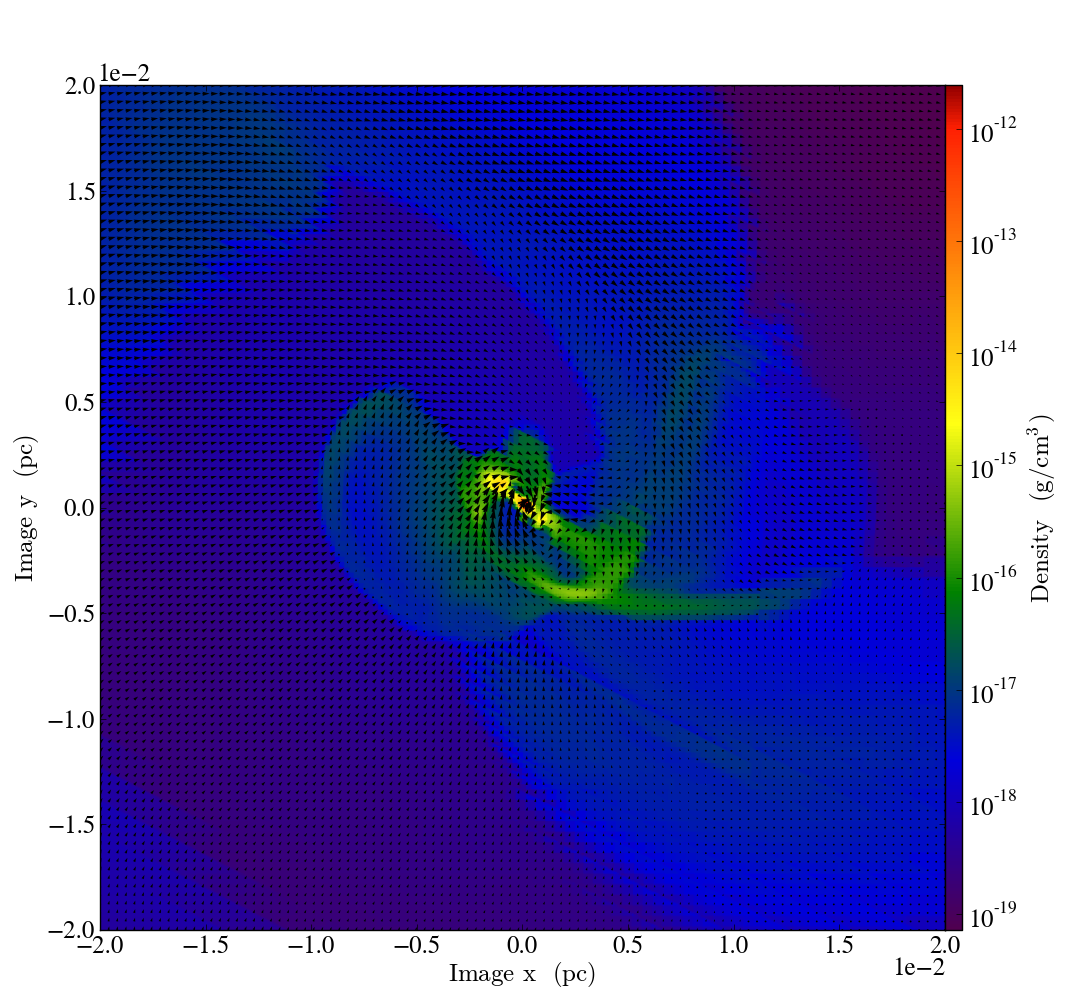
\includegraphics[width=0.48\textwidth]{movie_disk_0132_0002.png}
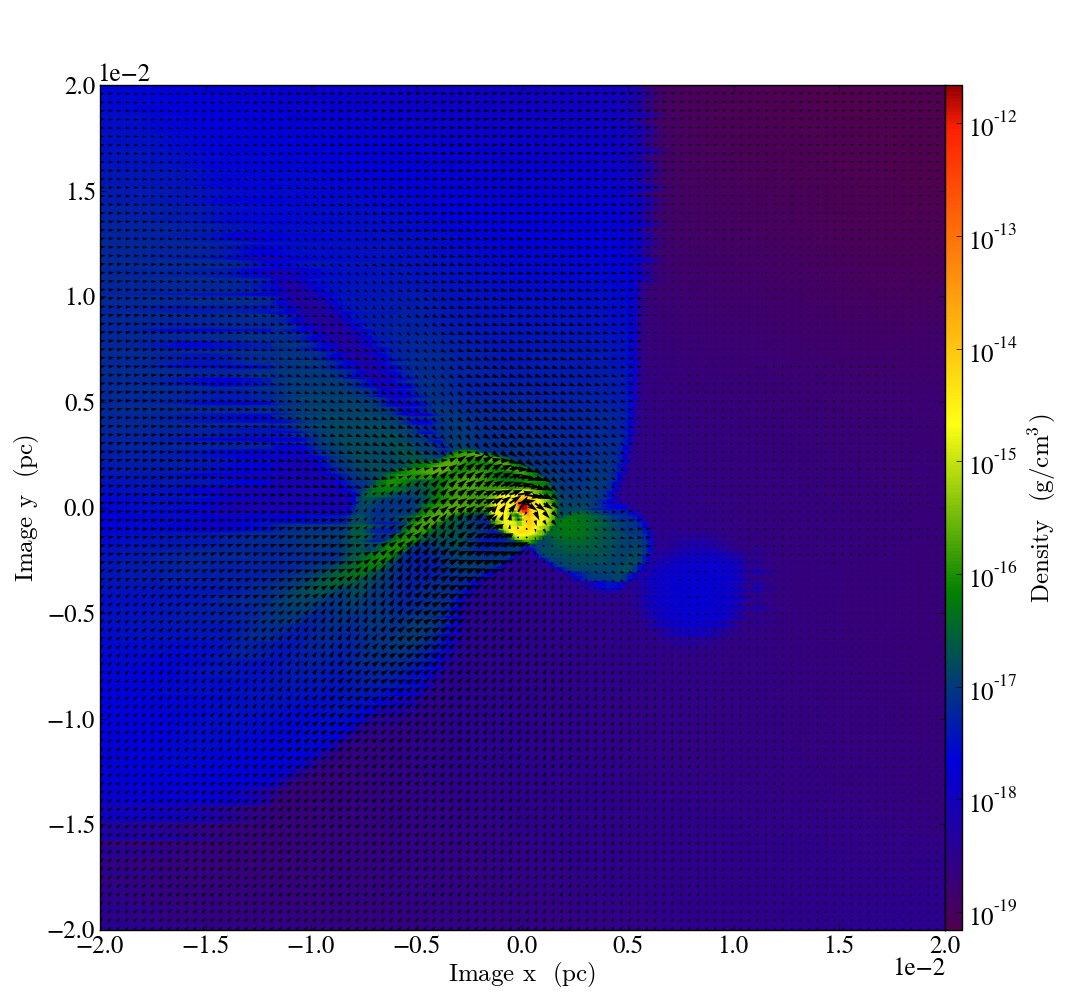
\includegraphics[width=0.48\textwidth]{movie_disk_0132_0004.png}
\centering{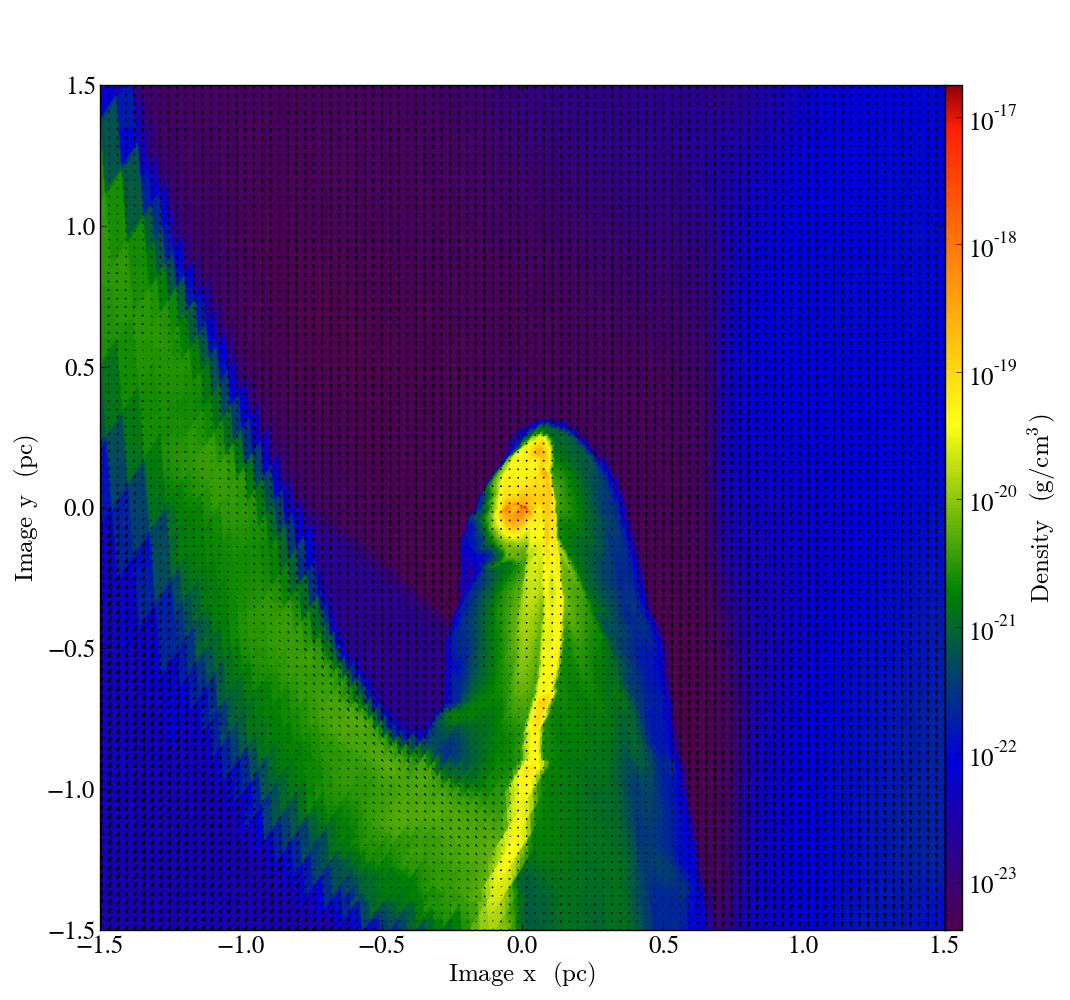
\includegraphics[width=0.48\textwidth]{Disk_0132_0002.png}}
\caption{{\bf Do same for other plots in 132} Slices along the angular momentum axis of four zoomed in simulation. To determine the angular momentum axis, we take a $0.01$ pc region about the densest local point and calculate the angular momentum vector. We then take a slice in the plane normal to the angular momentum to plot the regions around these dense points. \label{fig:snapshots 2}}
\end{figure*}

\begin{figure*}
\plottwo{Track_0132_000_rho.png}{pdf_frame_0132_0000.png}
\plottwo{Track_0132_000_vr.png}{Track_0132_000_mass.png}
\caption{Tracking 132 000  These plots show various data for one of the particles formed in the simulation.  The upper left graph shows the density profile, with reference lines indicating slopes of -3/2, -2, and -5/2.  The slope between $0.02$pc and $0.4$pc approximately matches the -5/2 reference line.  The plot on the upper right shows the pdf function related to volumes of 1pc, 2pc, and 5pc.  The bottom left shows a plot of the radial velocity and turbulent velocity associated with the particle.  The lower right graph shows the radial density profile of the particle.    \label{fig:132 000 graphs}}
\end{figure*}

\begin{figure*}
\plottwo{Track_0132_002_rho.png}{pdf_frame_0132_0002.png}
\plottwo{Track_0132_002_vr.png} {Track_0132_002_mass.png}
\caption{Tracking 132 002  These plots show the data for a different particle formed in the simulation at the same time as the previous plots.  The upper left graph of the density in the region neatly matches the -3/2 slope.  The pdf graph in the upper right again shows the plots for volumes related to $1$pc, $2$pc, and $5$pc.  The lower left plot demonstrates the loose connection between the radial velocity and the turbulent velocity.  The graph on the lower right again shows the density profile of this second particle.     \label{fig:132_002_graphs}}
\end{figure*}


The zoom in plots in Figures \ref{fig:snapshots} and \ref{fig:snapshots 2} suggest that the accretion can occur by streams or by spherical flows.  However, the degree by which these modes of accretion dominate, is not clear.  At small radii (similar to $10^{-2}$ pc), a protostellar disk appears in all four snapshots. The radial size of these disks varies. These disks also show a coherent sense of rotation about a common axis, e.g., no counter-rotating disks. In addition, some of the snapshots show multiple high density regions.  This could be a result of accretion of high density clumps or fragmentation in the disk or streams.  
 


\subsection{Examples of Collapse}

These simulations display much more complicated dynamics than is captured by the simple analytic theory of Murray and Chang 2014.  In spite of this, we compare radially averaged profiles around these high density points to their analytic theory.  In the left panel of Figure \ref{fig:good_rho_example}, we show the radial density profile around one such high density point. As this figure shows, the radial density profile follows a $r^{-3/2}$ power law in agreement with analytic expections.  This power-law breaks down at small radii, but this is not unexpected as this radii corresponds to the presents of a rotationally support disk.  Such good agreement is not universal for all high density points as shown in the right panel of Figure \ref{fig:bad_rho_example}.  Here the radial density profile follows a $r^{-2}$ power law.  
\begin{figure*}
\plottwo{Track_0256_000_rho.png}{Track_0132_000_rho.png}
\caption{Density as a function of radial position from maximum density point.  The density reaches a maximum of $10^6$ times mean density at $r \approx 10^{-3}$ pc and declines to approximately mean density at $r\approx 3$ pc.  The three straight solid lines are $r^{-3/2}$, $r^{-2}$, and $r^{-5/2}$ power laws. \label{fig:good_rho_example}
{bf\ This discusses left panel only, should we move the discussion outside the caption?}}
\end{figure*}


However, to make a comparison of the average behavior of high density star forming regions, we average over a number 

What plots should we show?
-velocities vs r
-angular momentum vs r
-mass vs r
-mdot vs r

In Figure \ref{fig:vr_example}, we plot $v_r$ (blue line) and $v_{\rm rms}$ (green line) as a function of $r$.  In the left panel, the radial velocity curve is sporadic, but the general trend is that $v_r$ declines in toward $0.1$ pc, but then rises inward of this point.  Plotted in red is a $r^{-1/2}$ power law and this inward rise appears to follow this general trend.  The turbulent velocity is smoother, but it follows the general trend of the $v_r$ curve in that it falls slowly inward toward $]\approx 0.1 $ pc before rising inward of that, roughly tracking the $r^{-1/2}$ power law.  These general trends are in rough agreement with our analytic expectations.  In the right panel, the radial velocity curve is smoother and increases inwards towards $0.01$ pc, tracking the $r^{-1/2}$ power law fairly closely.  This radial velocity begins to fall inward of $0.01$ pc, possibly due to rotational support from the angular momentum of a disk.  The turbulent velocity in the right panel seems to roughly follow an inverse relationship with the radial velocity.  As with the left panel, however, the turbulent velocity is significantly less volatile than the radial velocity and varies only slightly with $r$.   These expectations are in line with the analytic results of Murray and Chang (2014), albeit with a somewhat larger scale that they suggest.  
 
\begin{figure*}
\plottwo{Track_0256_000_vr.png}{Track_0132_000_vr.png}
\caption{Radial velocity, $v_r$ (blue line), and turbulent velocity, $v_{\rm rms}$ (green line) as a function of radial position from maximum density point.  A $r^{-1/2}$ power law is shown as a red line. \label{fig:vr_example}}
\end{figure*}

A hint of why these different behaviors emerge from looking at the $M(r)$.  In Figure \ref{fig:mass_example}, we plot the mass as a function of radius.  Regions where $M(r)$ flattens implies that the mass in this region can be treated using a point mass approximation.  Here it is apparent that the regions that can be treated a point mass corresponds to regions in where the density follows a $r^{-3/2}$ power law and the radial and turbulent velocities follow a $r^{-1/2}$ power law.  This is due to mass concentration at smaller radii as evident by the sudden drop in $M(r)$ at $r \approx 10^{-2} - 1$ pc.  The flattening of $M(r)$ on larger scales is interesting as this is due to the entire mass of the forming star cluster as opposed to the individual stars that MC14 originally envisioned.  Hence the entire mass of the star cluster contributes to the large scale dynamics of turbulent collapse.    

\begin{figure*}
\plottwo{Track_0256_000_mass.png}{Track_0132_000_mass.png}
\caption{WRITE CAPTION: Mass, $MSun$, as a function of radial position from a local maximum density point.     \label{fig:mass_example}}
\end{figure*}


\begin{figure*}
\plottwo{Track_0256_000_l.png}{Track_0132_000_l.png}
\caption{WRITE CAPTION: Mass, $MSun$, as a function of radial position from a local maximum density point.     \label{fig:angular_momentum_example}}
\end{figure*}

\begin{figure*}
\plottwo{pdf_frame_0256.png}{pdf_frame_0132.png}
\caption{Probability density function, $pdf$ as a function of density $rho/rho_0$.  \bf Verify range of slope calculation \label{fig:pdf_example}}
\end{figure*}

\begin{figure*}
\plottwo{Disk_0132_0000.png}{Disk_0132_0004.png}
\caption{Visualization of density profiles for two distinct particles in tracking1b. \label{fig:rho_example_132}}
\end{figure*}

\subsection{Average Profiles}

\section{Discussion and Conclusions}

\acknowledgments

Write

\begin{references}

\noindent
Bethe, H.~A. \& Salpeter, E.~E. 1957 \textit{Quantum Mechanics of One-
  and Two-Electron Atoms} (Berlin: Springer-Verlag) (BS) 

\noindent
Bildsten, L., Salpeter, E.~E. \& Wasserman, I. 1992, \apj, 384, 143
(BSW) 


\end{references}

\end{document}



